\documentclass{prova}

\usepackage{amsmath}
\usepackage{amsfonts}

\setlength{\textheight}{25cm}

\DeclareMathOperator{\sen}{sen}
\DeclareMathOperator{\tg}{tg}
\newcommand{\ds}{\displaystyle}

\professor{Prof.\@ Adriano Barbosa}
\disciplina{C\'alculo 2}
\avaliacao{P1}
\curso{Matem\'atica}
\data{17/08/2022}

\begin{document}
	\cabecalho{5}  % o numero 5 indica a qnt de quadros na tabela de nota

    \textbf{Todas as respostas devem ser justificadas.}

    \begin{questionario}
        \q{A velocidade de um corredor aumenta regularmente durante os tr\^es
           primeiros segundos de uma corrida. Sua velocidade em intervalos de
           meio segundo \'e dada pela tabela abaixo. Encontre as estimativas
           superior e inferior para a dist\^ancia que ele percorreu durante esses
           tr\^es segundos.}
            \begin{center}
            \begin{tabular}{|c|c|c|c|c|c|c|c|}
                \hline
                $t$ (s) & 0 & 0,5 & 1,0 & 1,5 & 2,0 & 2,5 & 3,0 \\
                \hline
                $v$ (m/s) & 0 & 1,9 & 3,3 & 4,5 & 5,5 & 5,9 & 6,2 \\
                \hline
            \end{tabular}
            \end{center}
        \q{Seja $F(x)=\ds\int_0^{x^4} \cos(t^2)\ dt$. Calcule $F'(x)$.}
        \q{Calcule a \'area da regi\~ao abaixo.}
            \begin{figure}[h]
                \centering
                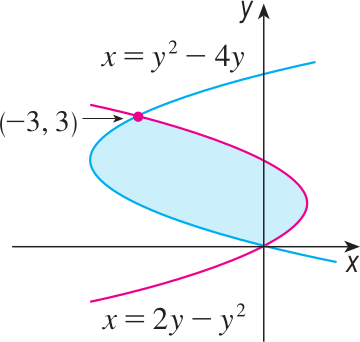
\includegraphics[width=0.3\textwidth]{fig01.png}
            \end{figure}
        \q{Calcule a integral $\ds\int \frac{\sen(\sqrt{x})}{\sqrt{x}}\
           dx$.}
        \q{Calcule o volume do s\'olido dado pela rota\c{c}\~ao da regi\~ao delimitada
           pelas curvas $y=2-\frac{1}{2}x$, $y=0$, $x=1$, $x=2$ em torno do eixo
           $x$.}
    \end{questionario}
\end{document}
